% Lesson 2

\chapter{Segunda Lección} % Chapter title

\label{ch:lesson02} % For referencing the chapter elsewhere, use \autoref{ch:examples} 

%----------------------------------------------------------------------------------------

\Large{\section{Gramática}}

\S\ 8. El estonio carece tanto de artículos definidos (`el', `la') como de artículos indefinidos (`un', `una'). Un sustantivo, como \textbf{poiss} `niño', puede significar tanto `niño', `un niño' o `el niño', dependiendo del contexto.\\

A veces el número \textbf{üks} `uno' puede servir como una especie de artículo indefinido, pero este uso es poco frecuente en el lenguaje escrito.\\

\Large{\section{El orden de las palabras}}

\S\ 9. A diferencia del español, donde el orden de las palabras puede presentar bastante complejidad, el estonio es bastante directo (sujeto - verbo - objeto): Poiss loeb raamatut `El niño lee un libro'.\\

Así mismo, el adjetivo precede al sustantivo que modifica en el estonio, a diferencia del español que puede aceptar el orden inverso. Ejemplos: \textbf{noor} poiss `el joven niño', \textbf{vana} mees `el viejo hombre'.\\

Un adverbio de tiempo por lo general precede a un adverbio de lugar en el estonio, en contraste con el español que acepta ambos ordenes: Ta tuleb \textbf{homme} siia `Él/Ella vendrá mañana aquí'. Poiss on \textbf{täna} kodus `El niño está hoy en casa'.\\

El orden inverso puede ser utilizado, con el verbo precediendo al sujeto, si la oración comienza con un adverbio o un objeto: Täna \textbf{on poiss} kodus `Hoy está el niño en casa'.\\

De lo contrario, no hay reglas estrictas para el orden de las palabras en una oración declarativa.\\

\S\ 10. Las preguntas suelen comenzar con una palabra especial o expresión interrogativa en el estonio. Luego el orden de las palabras es el mismo que en una frase ordinaria (especialmente si el sujeto es un pronombre personal).

\begin{center}
\begin{tabular}{ l l }
	Kus poiss elab? 	& `¿Dónde vive el niño?' (\emph{lit.} ¿Dónde el niño vive?) \\
	Mis see on?			& `¿Qué es eso?' (\emph{lit.} ¿Qué eso es?) \\
	Millal sa tuled? 	& `¿Cuándo vienes tú? (\emph{lit.} ¿Cuándo tú vienes?)
\end{tabular}\\ \bigskip
\end{center}

\S\ 11. Preguntas tales como `¿Estás leyendo?' `¿El niño viene?', que se puede responder ya sea con un `Sí' o un `No' y que equivalen a una afirmación con signos de interrogación en el español, comienzan con la palabra interrogativa especial \textbf{kas} en estonio, seguido por el orden normal de las palabras de una oración declarativa (en el español equivaldría a reemplazar el signo de interrogación `¿' por la palabra `kas').

\begin{center}
\begin{tabular}{ l l }
	Poiss loeb. 	& `El niño lee.' \\
	Kas poiss loeb? & `¿El niño lee?' \\
	Sina tuled.		& `Tú vienes' \\
	Kas sina tuled?	& `¿Tú vienes?' 
\end{tabular}\\ \bigskip
\end{center}

\S\ 12. En el lenguaje hablado y a veces incluso en el lenguaje escrito, puede que aparezcan preguntas que carecen de la palabra especial `kas' y tienen un orden inverso, como en el español: Tuled sa? `¿Vienes tú?' Oled sa kodus? `¿Estás tú en su casa?'\\

Al igual que en el español, una oración declarativa se puede convertir en una pregunta mediante una inflexión o cambio de tono en la voz, sin cambiar el orden de palabras:

\begin{center}
Sa tuled ju homme? `¿Tú vienes mañana?'\\
\end{center}

En el español, esto se hace mediante un incremento parcial y lineal del tono hasta el final de la frase. En el estonio, el tono se eleva en el centro (donde está el verbo) y vuelve a su nivel normal al final.\\

\S\ 13. Ocasionalmente, la respuesta afirmativa a las preguntas viene dada por el verbo de la pregunta, conjugado acorde al sujeto implícito. A menudo se da énfasis con la palabra \textbf{küll} `ciertamente'. 

\begin{center}
\begin{tabular}{ l l }
	Kas sa \textbf{oled} kodus? & `¿Estás en casa?'\\
	\textbf{Olen küll.}			& `(Ciertamente) sí estoy'\\
	Kas te \textbf{tulete}? 	& `¿Ustedes vienen?'\\
	\textbf{Tuleme küll.}		& `(Ciertamente) sí venimos'
\end{tabular}\\ \bigskip
\end{center}

\section*{\Large{Texto}}

Kes see on? See on poiss. Kes seal on? Seal on tüdruk. Mis see on? See on laud. Seal on tool. Kas poiss istub? Poiss seisab, aga tüdruk istub. Mis nad teevad? Nad räägivad. Kas teie ka räägite? Meie õpime. Kus te olete? Me oleme siin. Kus tema on? Ta on seal. Mis ta teeb? Ta loeb ja kirjutab. Kas sa tead, mis see on? Tean küll, see on tool. Kas te teate, kus ta elab? Teame küll, ta elab siin.\\

—	Hallo, kes räägib? \\
—	Siin olen mina. \\
—	Kas sa oled täna kodus? \\
—	Jah, olen küll. \\
—	Kas sa tuled homme? \\
—	Jah, ma tulen. \\
—	Mis sa teed? \\
—	Õpin! \\
—	Kuidas läheb? \\
—	Tänan, hästi. \\
—	See on tore. \\

\begin{center}
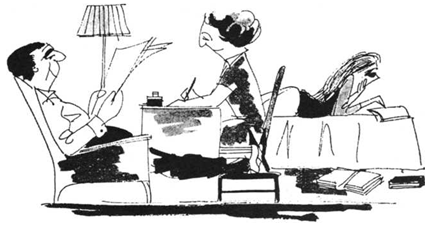
\includegraphics{img/L02.png}
\end{center}

Isa on täna kodus. Ta istub ja loeb. Ema on ka siin. Ta kirjutab. Tütar õpib. Poeg tuleb ja küsib: \guillemotleft Mis te siin teete?\guillemotright Õde vastab: \guillemotleft Armas vend, sa näed ju ise: me istume, õpime, loeme ja kirjutame.\guillemotright\\

\section*{\Large{Vocabulario}}

\begin{tabular}{ l l }
	aga				& pero \\
	armas			& querido/a \\
	ema				& madre \\
	hallo			& hola \\
	isa				& padre \\
	ise				& mismo (yo mismo, tú mismo, etc.) \\
	istu/n			& (yo) me siento  \\
	jah				& sí \\
	ju				& por supuesto \\
	kas				& interrogación \\
	kes				& quién \\
	kuid			& aunque, pero \\
	kuidas			& cómo \\
	kuidas läheb?	& ¿cómo va? \\
	kus				& dónde \\
	küll			& ciertamente \\
	küsi/n			& (yo) pregunto \\
	laud			& mesa, pizarra \\
	loe/n			& (yo) leo \\
	lähe/n			& (yo) voy \\
	mis				& qué \\
	näe/n			& (yo) veo \\
	poeg			& hijo \\
	poiss			& niño \\
	see				& esto \\
	seisa/n			& (yo) me paro \\
	tea/n			& (yo) sé \\
	tee/n			& (yo) hago \\
	tool			& silla \\
	tore			& bien, fabuloso, divertido \\
	tüdruk			& niña \\
	tütar			& hija \\
	vasta/n			& (yo) respondo \\
	vend			& hermano \\
	õde				& hermana
\end{tabular}\\ \bigskip

\section*{\Large{Ejercicios}}

\begin{enumerate}
	\item \emph{Conjugue los siguientes verbos en estonio en tiempo presente:} hacer, saber, preguntar, responder, sentarse, pararse.
	\item \emph{Traducir al estonio:} ¿Dónde vives? ¿Quién está preguntando? ¿Estás en casa? ¿Dónde están? ¿Qué están haciendo aquí? Estamos sentados y hablando. ¿Está el niño parado? Sí, él está parado aquí. ¿Qué está haciendo la niña? La niña está sentada y leyendo. ¿Qué es esto? ¿Ustedes saben? ¿Tú sabes qué es esto? El hermano está aquí, pero la hermana está ahí. ¿Dónde está papá? ¿Qué está haciendo mamá? Yo voy a preguntar, y tú vas a responder. ¡Por favor (acepte esto)! ¡Muchas gracias!
	\item \emph{Traduzca al español:} Kas sa tuled homme? Kes seal on? Kus sa elad? Kuidas läheb? Mis see on? 
\end{enumerate}

\section*{\Large{Expresiones de preocupación}}

\begin{tabular}{ l p{6.5cm} }
	Kuidas käsi käib?				& ¿Cómo estás? (\emph{lit.} ¿Cómo va la mano?) \\
	Kuidas läheb?					& ¿Cómo va? \\
	Kuidas elad? Kuidas elate?		& ¿Cómo te sientes? (\emph{lit.} ¿Cómo estás/está viviendo?) \\
	Tänan, hästi.					& Bien, gracias. \\
	Kuidas ise elate?				& ¿Cómo se siente usted? \\
	Suur tänu, kõik on hästi.		& Muchas gracias, todo está bien. (\emph{lit.} Grande gracias, todo está bien.) \\
	Aitäh, pole viga.				& Gracias, no hay problemas. \\
	Halvasti.						& Mal. \\
	Mis sa soovid? Mida te soovite? & ¿Qué deseas? ¿Qué desean? \\
	Kas te soovite (midagi)?		& ¿Desean algo? \\
	Jah, palun. Ei, tänan.			& Sí, por favor. No, gracias. \\
	Kas jah või ei?					& ¿Sí o no?
\end{tabular}\\ \bigskip

\section*{\Large{Respuesta a los ejercicios}}

\begin{enumerate}
\item
\begin{tabular}{ l l l l l l l }
(ma)	& teen		& tean		& küsin		& vastan	& istun		& seisan \\
(sa)	& teed		& tead		& küsid		& vastad	& istud		& seisad \\
(ta)	& teeb		& teab		& küsib		& vastab	& istub		& seisab \\
(me)	& teeme		& teame		& küsime	& vastame	& istume	& seisame \\
(te)	& teete		& teate		& küsite	& vastate	& istute	& seisate \\
(nad)	& teevad	& teavad	& küsivad	& vastavad	& istuvad	& seisavad
\end{tabular}
\item Kus sa elad? Kes küsib? Kas (sa) oled kodus? [= Oled (sa) kodus?] Kus nad on? Mis te siin teete? [= Mis te teete siin?] Me istume ja räägime. Kas poiss seisab? Jah, ta seisab siin. Mis tüdruk teeb? [= Mis teeb tüdruk?] Tüdruk istub ja loeb. Mis see on? Kas (te) teate? Kas sa tead, mis see on? Vend on siin, aga [= kuid] õde on seal. Kus isa on? Mis ema teeb? Mina küsin, ja sina vastad. Palun! Tänan väga!
\item ¿Vienes mañana? ¿Quién está ahí? ¿Dónde vives? ¿Cómo va? ¿Qué es esto?
\end{enumerate}
%----------------------------------------------------------------------------------------